\documentclass{report}
\usepackage[a4paper, total={7.5in, 10in}]{geometry}
\usepackage{polski}
\usepackage[utf8]{inputenc}
\usepackage{amsmath}
\usepackage{amssymb}
\usepackage{graphicx}
\usepackage{float}
\usepackage{amsfonts}
\usepackage{sectsty}
\usepackage{titlesec}
\usepackage{setspace}
\usepackage{booktabs}
\usepackage{stix}
\usepackage{fancyhdr}
\usepackage{hyperref}
\usepackage{caption}

\usepackage{enumitem}
\usepackage{pgfplots}
\usepackage{etoolbox}
\usepackage{subcaption}
\usepackage{multirow}
\usepackage{xcolor}
\usepackage{enumitem}
\graphicspath{ {zdj} }
\pagestyle{empty}

\setlength{\parindent}{0pt}

\newcommand\setItemnumber[1]{\setcounter{enumi}{\numexpr#1-1\relax}}



\titlespacing*{\chapter}{0pt}{-35pt}{0pt}
\titlespacing*{\section}{0pt}{-20pt}{10pt}
\titlespacing*{\subsection}{0pt}{-20pt}{10pt}
\titlespacing*{\subsubsection}{0pt}{0pt}{10pt}

\titleformat{\chapter}[display]{\normalfont\Large\bfseries\filcenter}{}{10pt}{\Large}
\titleformat{\section}[display]{\normalfont\large\bfseries\filcenter}{}{10pt}{\large}
\titleformat{\subsection}[display]{\normalfont\normalsize\bfseries\filcenter}{}{10pt}{\normalsize}
\titleformat{\subsubsection}[display]{\normalfont\small\bfseries}{}{10pt}{\small}

\setcounter{tocdepth}{3}
\setcounter{secnumdepth}{3}

\pagestyle{fancy}
\fancyhf{}
\fancyfoot[R]{Strona \thepage}
\renewcommand{\headrulewidth}{1pt}
\renewcommand{\footrulewidth}{1pt}
\fancypagestyle{plain}{\pagestyle{fancy}}

\fancyfoot[L]{Popławski Dawid}%
\fancyhead[R]{}%


\DeclareCaptionFormat{custom}
{%
	\textbf{#1#2}\textit{\small #3}
}
\renewcommand{\figurename}{Rys.}

\captionsetup{format=custom,%
				margin={5pt,5pt},%
				justification=centering}
\usepackage[T1]{fontenc}       % change font encoding to T1
\usepackage[framed,numbered]{matlab-prettifier}



\begin{document}
	\begin{titlepage}
		\begin{figure}[h]
			\begin{minipage}[l]{.5\textwidth}%
				
\includegraphics[width=0.3\textwidth]{pwr_logo}
			\end{minipage}%
			\begin{minipage}[r]{.5\textwidth}%
				
\includegraphics[width=1\textwidth]{wit_logo}
			\end{minipage}%
		\end{figure}
		
		\vspace*{3mm}
		
		\begin{center}
			\rule{\textwidth}{0.8pt}\\ 
			\vspace*{6mm}
			{\LARGE Platformy programistyczne .Net i Java - LAB2}\\
			\vspace*{3mm}
			\rule{\textwidth}{0.8pt}\\
			
			\vspace{1.5cm}
			{\setstretch{2}
				Politechnika Wrocławska
				
				Wydział Informatyki i telekomunikacji
				
				Kierunek: Informatyczne systemy automatyki
				
				grupa nr 2
				
				\href{https://github.com/wernexnrs/264254-.NET-i-Java}{github.com/wernexnrs/264254-.NET-i-Java}
				
			}
		\end{center}
		
		\vspace*{2cm}
		
		\begin{flushright}
			{\setstretch{2}
				Dawid Popławski - $264254$
				
				Termin zajęc: Środa godz. $17^{\underline{05}}$ - $18^{\underline{45}}$ 
				
				Prowadzący: mgr inż. Michał Jaroszczuk
				
			}
			
		\end{flushright}
		
		\vfill
		
\end{titlepage}

\tableofcontents

\chapter{Opis programu}

Kod przedstawia aplikację w Windows Forms napisaną w C\#, która służy do wizualizacji danych pogodowych. Aplikacja pobiera informacje o pogodzie z zewnętrznego API (OpenWeatherMap), wyświetla je użytkownikowi i zapisuje w lokalnej bazie danych SQLite. Baza danych SQLite jest strukturyzowana w taki sposób, aby przechowywać dane pogodowe wraz z powiązanymi informacjami, takimi jak współrzędne (szerokość i długość geograficzna), warunki pogodowe, szczegóły wiatru, informacje systemowe (np. kraj, czasy wschodu i zachodu słońca) oraz zachmurzenie. Entity Framework Core jest używany do mapowania tych jednostek danych na bazę danych.

\vspace*{15pt}

{\let\clearpage\relax\chapter{Struktura Projektu}}

\begin{itemize}
	\item Form1.cs: Główny formularz aplikacji, zawierający interfejs użytkownika i logikę interakcji z danymi pogodowymi.
	
	\item Json\_data.cs: Definiuje model danych oraz kontekst bazy danych do interakcji z lokalną bazą danych SQLite.
\end{itemize}

\begin{figure}[H]%
	\centering
	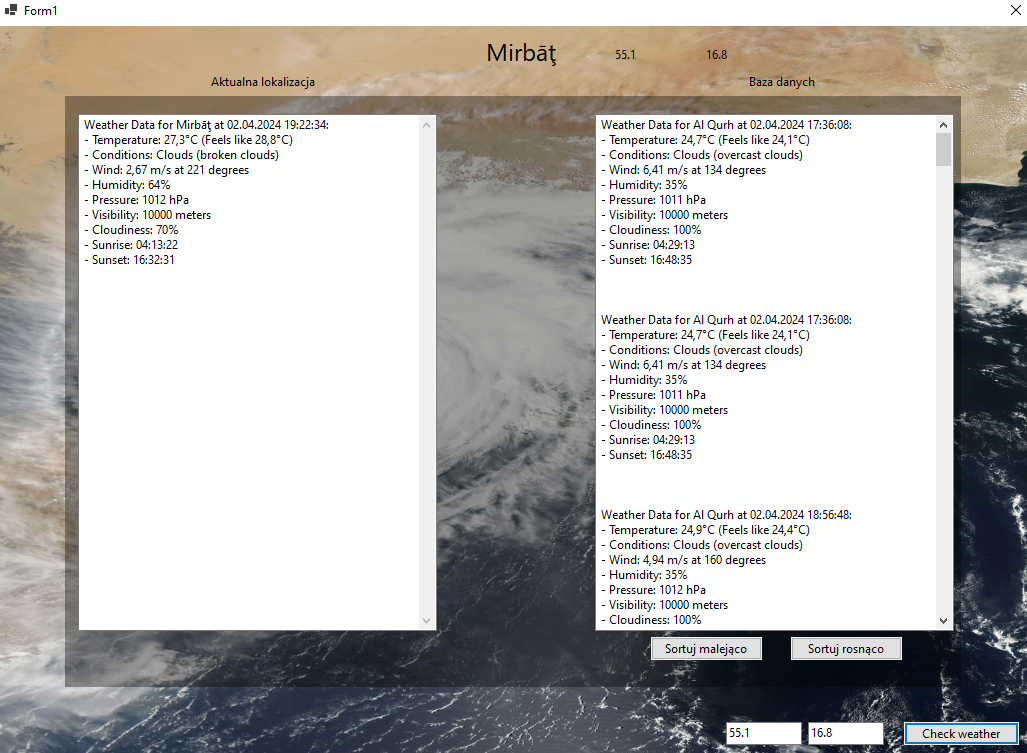
\includegraphics[scale=0.6]{zdj/main}
	\caption{Wynik programu.}
\end{figure}
\end{document}